\documentclass[10pt]{beamer}

\usetheme{metropolis}
\usepackage[utf8]{inputenc}
\usepackage[brazilian]{babel}

\usepackage{booktabs}
\usepackage[scale=2]{ccicons}
\usepackage{listings}

\usepackage{pgfplots}
\usepgfplotslibrary{dateplot}

%Justificar texto
\usepackage{ragged2e}
\addtobeamertemplate{block begin}{}{\justifying}

\usepackage{xspace}
\newcommand{\themename}{\textbf{\textsc{metropolis}}\xspace}

\usepackage{tikz}
\usetikzlibrary{shapes,arrows}

\title{Projeto e Implementação em Controlador Industrial para Posicionamento de Risers com Validação Experimental}
%\subtitle{A modern beamer theme}
\date{\today}
\author{Ataias Pereira Reis\\ Emanuel Pereira Barroso Neto}
\institute{Faculdade de Tecnologia\\ Universidade de Brasília}
 \titlegraphic{\hfill
\includegraphics[height=1.0cm]{figures/logoVerdeUnB}}
 
 \newcommand\Fontvi{\fontsize{6}{7.2}\selectfont}

\begin{document}

\maketitle

\begin{frame}{Índice}
  \setbeamertemplate{section in toc}[sections numbered]
  \tableofcontents[hideallsubsections]
\end{frame}

\section{Introdução}

\begin{frame}[fragile]{Risers}

\begin{columns}[T] % align columns
\begin{column}{.5\textwidth}
%\color{red}\rule{\linewidth}{4pt}

\begin{block}{}
\begin{itemize}
\item Há diversas operações realizadas em plataformas de petróleo em alto mar. Entre elas, a operação de reentrada dos risers. Este procedimento é muitas vezes realizado manualmente. \item A proposta deste trabalho é mostrar que é possível fazer isso de forma automática, por meio de testes em bancada laboratorial, utilizando técnicas de controle para sistemas de ordem infinita.
\end{itemize}\end{block}

\end{column}%
\hfill%
\begin{column}{.5\textwidth}
%\color{blue}\rule{\linewidth}{4pt}

\begin{figure}[!ht]
\centering
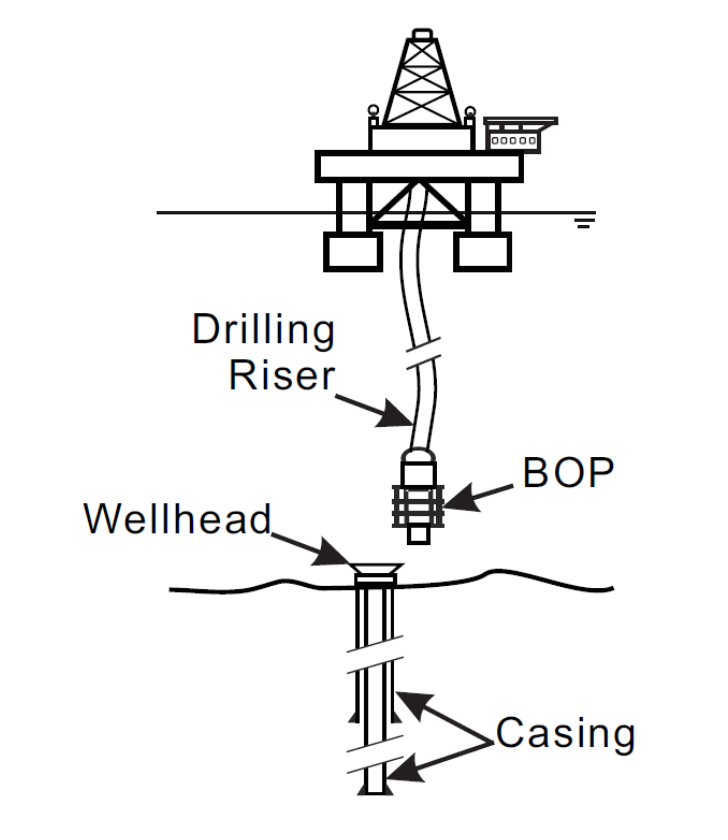
\includegraphics[width=1\linewidth]{figures/introducao/riser}
\caption{Operação de Reentrada \cite{redytton}}
\end{figure}

\end{column}%
\end{columns}

\end{frame}
\begin{frame}[fragile]{Risers}
  \begin{columns}[T] % align columns
\begin{column}{.5\textwidth}
%\color{red}\rule{\linewidth}{4pt}

\begin{figure}[!ht]
\centering
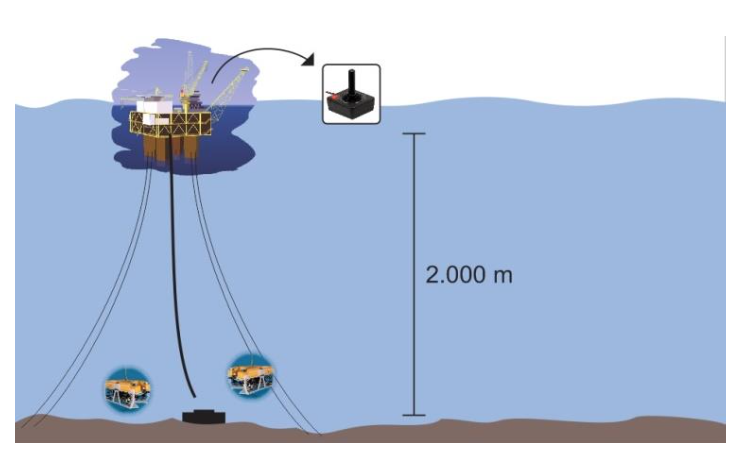
\includegraphics[width=1\linewidth]{figures/introducao/posicionamentoAtual}
\caption{Método atual para reconexão no poço \cite{redytton}}
\end{figure}


\end{column}%
\hfill%
\begin{column}{.5\textwidth}
%\color{blue}\rule{\linewidth}{4pt}

\begin{figure}[!ht]
\centering
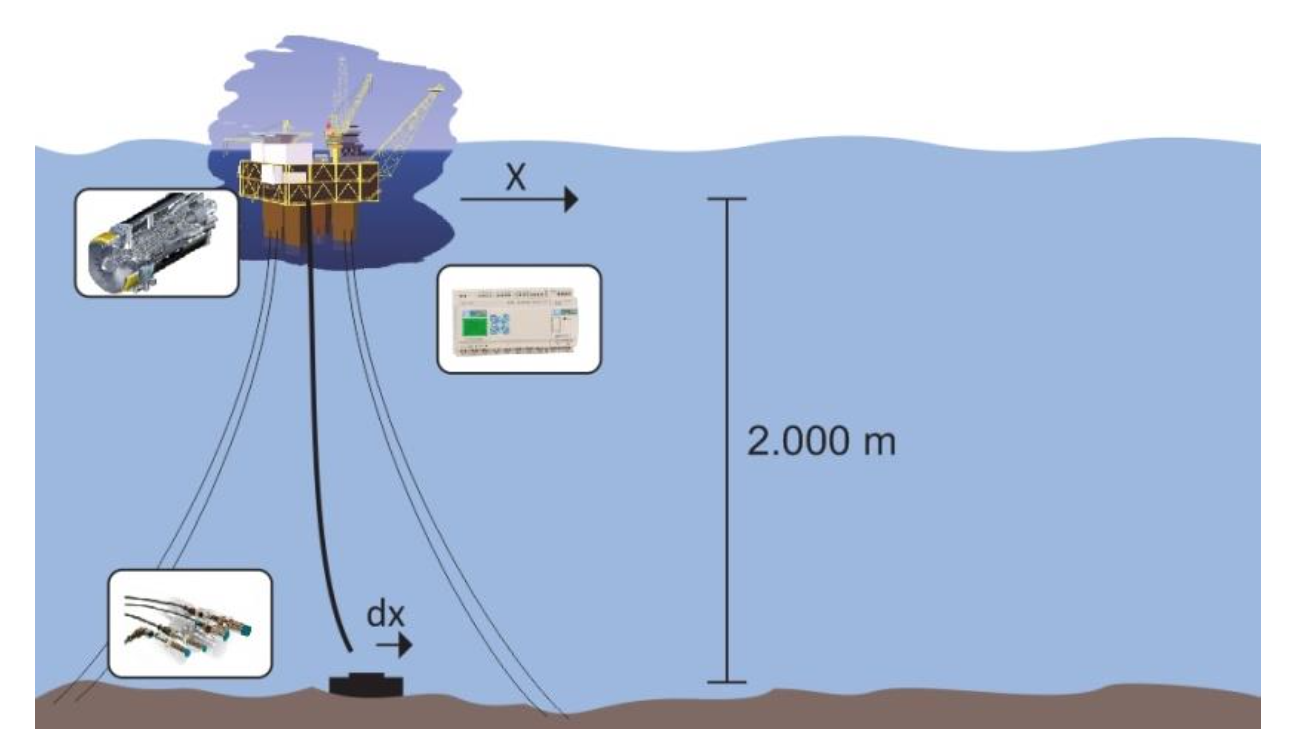
\includegraphics[width=1\linewidth]{figures/introducao/posicionamentoProposto}
\caption{Método proposto para reconexão no poço \cite{redytton}}
\end{figure}

\end{column}%
\end{columns}

\end{frame}

\section{Fundamentos}

\begin{frame}[fragile]{Equações Governantes}

\begin{block}{}
Utiliza-se a simplificação de Euler-Bernoulli para vigas, uma vez que \textit{risers} são esbeltos e possuem alto módulo de cisalhamento.
\end{block}

\begin{block}{}
A equação diferencial parcial para a variável deslocamento, $\Upsilon$, é dada por \begin{align}
	m_s \frac{\partial^2 \Upsilon}{\partial t^2} &= -E J	\frac{\partial^4 \Upsilon}{\partial z^4} + \frac{\partial}{\partial z}\left(T(z) \frac{\partial \Upsilon}{\partial z}\right) + F_n(z,t),
\end{align} na qual $m_s$ é a densidade linear do tubo, $E$ é o módulo de Young e $J$ é o segundo momento de inércia do \textit{riser}. $T(z)$ descreve as forças de tração ao longo do comprimento do \textit{riser}. $F_n(z,t)$ é a força resultante externa \cite{fabricioIFAC}.
\end{block}

\end{frame}

\begin{frame}[fragile]{Equações Governantes}
\begin{block}{Equação de Morison}
\begin{align}
	F_n(z,t) &= -m_{fbar} \frac{\partial^2 \Upsilon}{\partial t^2} - \mu \left|\frac{\partial \Upsilon}{\partial t}\right|\frac{\partial \Upsilon}{\partial t}\label{forceN}
\end{align}
\end{block}
\begin{block}{Equação completa para o deslocamento do barbante}
\begin{align}
	\frac{\partial^2 \Upsilon}{\partial t^2} &= -\frac{EJ}{m}\frac{\partial^4 \Upsilon}{\partial z^4} + \frac{\partial}{\partial z}\left(\frac{T(z)}{m}\frac{\partial \Upsilon}{\partial z}\right) - \frac{\mu}{m}\left|\frac{\partial \Upsilon}{\partial t}\right|\frac{\partial \Upsilon}{\partial t}\label{equacaoBarbante}
	\end{align}
\end{block}
\begin{block}{}
\begin{itemize}
	\item $\mu$ é o coeficiente de arrasto (unidade 1/s) 
	\item $m_{fbar}$ é a massa do fluido adicionado
	\item $m = m_s + m_{fbar}$
\end{itemize}	
\end{block}
\end{frame}

\begin{frame}[fragile]{Equações Governantes}
\begin{block}{Equação para o deslocamento da carga}
	\begin{align}
 	\ddot{\Upsilon}_1 &= b_1\left(-\Upsilon_1 + \Upsilon_2\right) - \tau'\dot{\Upsilon}_1\label{upsilon1final}
 \end{align}
\end{block}

\begin{itemize}
	\item $b_1 = \frac{m_b g}{m'l} = \frac{g}{l}$
	\item $\tau'$ é a linearização do termo $\frac{1}{2m_b}\rho C_d A_b \left|\dot{\Upsilon}_1\right|$
\end{itemize}
	
\end{frame}

\begin{frame}[fragile]{Discretização}

\begin{block}{}
\begin{itemize}
	\item A equação \ref{equacaoBarbante} é uma EDP em $z$ e precisa ser discretizada. No presente trabalho, utilizou-se o método diferenças finitas para discretizar em $z$.
\end{itemize}
\end{block}

\begin{block}{$k$-ésima EDO}
\begin{align}
	\frac{d^2\Upsilon_k}{dt^2} &= -\frac{EJ}{m l\,^4}\left(\Upsilon_{k-2} - 4\Upsilon_{k-1}+6\Upsilon_{k}-4\Upsilon_{k+1}+\Upsilon_{k+2}\right)\nonumber\\
	&+ \frac{T_0+mg(k-1)l}{m l\,^2}\left(\Upsilon_{k-1}-2\Upsilon_{k} + \Upsilon_{k+1}\right)+g\frac{-\Upsilon_{k-1}+\Upsilon_{k+1}}{2l}\nonumber\\
	&-\tau\frac{d\Upsilon_k}{dt}
\end{align}
\end{block}
\end{frame}

\begin{frame}[fragile]{Definição de constantes}
\begin{align}
	a &= -\frac{EJ}{m l^4}\\
	b_k &= \frac{T_0 + mg(k-1)l}{m l^2},\; k\ge 2\\
	c &= \frac{g}{2l}\\
	d_k &= b_k - c,\; k\ge 2\\
	e_k &= b_k + c,\; k\ge 2
\end{align}	
\end{frame}

\begin{frame}[fragile]{Caso exemplo de espaço de estados}
\begin{block}{Definição dos estados, entrada e saída}
	\begin{align}
	\begin{array}{ll}
	\mathbf{x} &= \left(\Upsilon_1\;\Upsilon_2\;\Upsilon_3\;\Upsilon_4\;\Upsilon_5\;\Upsilon_6\;\dot{\Upsilon}_1\;\dot{\Upsilon}_2\;\dot{\Upsilon}_3\;\dot{\Upsilon}_4\;\dot{\Upsilon}_5\;\dot{\Upsilon}_6\right)^T\\
	u &= \Upsilon(L,t) = \Upsilon_7\\
	y &= \Upsilon(0,t) = \Upsilon_1
\end{array}
 \end{align} 
\end{block}

\begin{block}{Equações para as derivadas segundas}
\begin{align}
	\ddot{\Upsilon}_1 &= b_1\left(-\Upsilon_1 + \Upsilon_2\right) - \tau'\dot{\Upsilon}_1\\
	\ddot{\Upsilon}_i &=d_i\Upsilon_{i-1} - 2b_i \Upsilon_{i} + e_i\Upsilon_{i+1} - \tau \dot{\Upsilon}_i,\; 2\le i \le 5\\
	\ddot{\Upsilon}_6 &= d_6\Upsilon_5 - 2b_6 \Upsilon_6 + e_6 u - \tau \dot{\Upsilon}_6
\end{align}	
\end{block}
\end{frame}

\begin{frame}[fragile]{Espaço de Estados}
\Fontvi
	\begin{align}
 	\dot{\mathbf{x}} &= \left[\begin{array}{cccccccccccc}
 		0 & 0 & 0 & 0 & 0 & 0 & 1 & 0 & 0 & 0 & 0 & 0\\
 		0 & 0 & 0 & 0 & 0 & 0 & 0 & 1 & 0 & 0 & 0 & 0\\
 		0 & 0 & 0 & 0 & 0 & 0 & 0 & 0 & 1 & 0 & 0 & 0\\
 		0 & 0 & 0 & 0 & 0 & 0 & 0 & 0 & 0 & 1 & 0 & 0\\
 		0 & 0 & 0 & 0 & 0 & 0 & 0 & 0 & 0 & 0 & 1 & 0\\
 		0 & 0 & 0 & 0 & 0 & 0 & 0 & 0 & 0 & 0 & 0 & 1\\
 		-b_1 & b_1 & 0 & 0 & 0 & 0 & -\tau' & 0     & 0 & 0 & 0 & 0\\
 		d_2 & -2b_2  & e_2  & 0  & 0 & 0 &  0    & -\tau & 0 & 0 & 0 & 0\\
 		0 & d_3 & -2b_3  & e_3  & 0  & 0 & 0 &  0    & -\tau & 0 & 0 & 0\\
 		0 & 0 & d_4 & -2b_4  & e_4  & 0  & 0 & 0 &  0    & -\tau & 0 & 0\\
 		0 & 0 & 0 & d_5 & -2b_5  & e_5  & 0  & 0 & 0 &  0    & -\tau & 0\\
 		0 & 0 & 0 & 0 & d_6 & -2b_6  & 0  & 0 & 0 &  0    & 0   &-\tau\\
 	\end{array}\right]\mathbf{x} \nonumber\\
 	&+ \left[0\;0\;0\;0\;0\;0\;0\;0\;0\;0\;0\;e_6\right]u
 \end{align}
\end{frame}

\begin{frame}[fragile]{Espaço de Estados}
Para o caso de uma discretização com $N$ pontos, tem-se 
\begin{align}
\begin{array}{ll}
 	\dot{\mathbf{x}} &= \left[\begin{array}{cc}
	\mathbf{0}_{N\times N} & \mathbf{I}_{N\times N}\\
	\mathbf{M}_{N\times N} & \mathbf{L}_{N\times N}\\
\end{array}\right] \mathbf{x} + \left[\begin{array}{c}
	\mathbf{0}_{2N-1\times 1}\\ e_N\\
\end{array} \right]u,\;\;\\
y &= \left[\begin{array}{cc}
	1 & \textbf{0}_{1\times 2N-1}
\end{array}\right]\textbf{x}.
\end{array}
 \end{align}

\end{frame}



\begin{frame}[fragile]{Constantes da planta}

\begin{block}{}
\begin{table}[!ht]
	\centering
	\caption{Constantes do barbante\label{constanteBarbante}}
	\begin{tabular}{|l|c|c|c|}
		\hline
		\textbf{Significado} & \textbf{Símbolo} & \textbf{Valor} & \textbf{Unidade}\\ \hline \hline
		Massa & $m_{bar}$ & 0.492 & g\\ \hline
		Comprimento & $L$ & 0.82 & m \\ \hline
		Massa linear & $m_s$ & 0.6 & g/m\\ \hline
		Raio & $r_{bar}$ & 1 & mm\\ \hline
		Densidade & $\rho_{bar}$ & 191 & kg/m$^3$\\ \hline
		Termo de arrasto linear & $\tau$ & 0.2426 & 1/s\\ \hline
	\end{tabular}
	
\end{table}

\end{block}

\begin{block}{}
\begin{itemize}
	\item O termo $\tau$ foi obtido considerando-se uma excursão de 30cm e é a média do termo $\frac{\mu}{m}\left|\frac{\partial \Upsilon}{\partial t}\right|$
\end{itemize}	
\end{block}


\end{frame}


\begin{frame}[fragile]{Constantes da planta}

\begin{block}{}
\begin{table}[!ht]
	\centering
	\caption{Constantes da bolinha de isopor\label{constanteIsopor}}
	\begin{tabular}{|l|c|c|c|}
		\hline
		\textbf{Significado} & \textbf{Símbolo} & \textbf{Valor} & \textbf{Unidade}\\ \hline \hline
		Massa & $m_{b}$ & 0.492 & g\\ \hline
		Raio & $r_{b}$ & 15.3 & mm\\ \hline
		Coeficiente de inércia & $C_m$ & 1.2 & - \\ \hline
		Coeficiente de arrasto & $C_d$ & 0.6 & - \\ \hline
		Volume & $V_b$ & $\frac{4}{3}\pi r_b^3$ & $\textrm{m}^3$ \\ \hline
		Área da seção transversal & $A_b$ & $\pi r_b^2$ & m$^2$\\ \hline
		Termo de arrasto linear & $\tau'$ & 0.1133 & 1/s\\ \hline
	\end{tabular}
	
\end{table}

\end{block}	
\end{frame}




\begin{frame}[fragile]{Controle - Malha Aberta x Malha Fechada}

\tikzstyle{block} = [draw, fill=blue!20, rectangle,font=\tiny, 
minimum height=0.5em, minimum width=1em]
\tikzstyle{sum} = [draw, fill=blue!20, circle, node distance=1cm]
\tikzstyle{input} = [coordinate]
\tikzstyle{output} = [coordinate]
\tikzstyle{pinstyle} = [pin edge={to-,thin,black}]

\begin{columns}[T,onlytextwidth]

\begin{column}{.5\textwidth}

\begin{figure}[!ht]
	
	%\centering
	% The block diagram code is probably more verbose than necessary
	\begin{tikzpicture}[auto, node distance=1cm,>=latex']
	% We start by placing the blocks
	\node [input, name=input] {};
	\node [block, right of=input] (controller) {Controlador};
	\node [block, right of=controller, pin={[pinstyle,font=\small]above:Perturbações},
	node distance=2cm] (system) {Planta};
	% We draw an edge between the controller and system block to 
	% calculate the coordinate u. We need it to place the measurement block. 
	\draw [->] (controller) -- node[name=u] {$u$} (system);
	\node [output, right of=system] (output) {};
	
	% Once the nodes are placed, connecting them is easy. 
	\draw [draw,->] (input) -- node {$r$} (controller);
	\draw [->] (system) -- node [name=y] {$y$}(output); 
	\end{tikzpicture}
	\caption{Malha aberta de controle\label{mabertatikz}}
\end{figure}


\begin{figure}[!ht]
\centering
% The block diagram code is probably more verbose than necessary

\begin{tikzpicture}[auto, node distance=1cm,>=latex']
% We start by placing the blocks
\node [input, name=input] {};
\node [sum, right of=input] (sum) {};
\node [block, right of=sum] (controller) {Controlador};
\node [block, right of=controller, pin={[pinstyle,font=\small]above:Perturbações},
node distance=1.5cm] (system) {Planta};
% We draw an edge between the controller and system block to 
% calculate the coordinate u. We need it to place the measurement block. 
\draw [->] (controller) -- node[name=u] {$u$} (system);
\node [output, right of=system] (output) {};
\node [block, below of=u] (measurements) {Medição};

% Once the nodes are placed, connecting them is easy. 
\draw [draw,->] (input) -- node {$r$} (sum);
\draw [->] (sum) -- node {$e$} (controller);
\draw [->] (system) -- node [name=y] {$y$}(output);
\draw [->] (y) |- (measurements);
\draw [->] (measurements) -| node[pos=0.99] {$-$} 
node [near end] {$y_m$} (sum);
\end{tikzpicture}
\caption{Malha fechada de controle\label{mfechadatikz}}
\end{figure}
\end{column}

\begin{column}{.5\textwidth}

\begin{block}{Controle em Malha Aberta}
Saída não é realimentada - não necessita do uso de sensores.
\newline
\newline
\newline
\end{block}

\begin{block}{Controle em Malha Fechada}
Possui realimentação - obtém o sinal de referência para a planta pela evolução do erro.\end{block}

\end{column}

\end{columns}
\end{frame}


\begin{frame}[fragile]{Preditor de Smith}
\begin{block}{Sobre o Preditor}
\begin{itemize}
\item Pode ser visto como um compensador de atraso;
\item Permite o projeto de controladores no sistema reduzido desconsiderando-se o atraso, tornado possível o uso de técnicas simples de controle no espaço de estados.
\end{itemize}
\end{block}
\end{frame}

\begin{frame}[fragile]{Estrutura do Preditor de Smith}
Na Figura \ref{smithStruct1}, \textbf{P} é a planta, \textbf{C} é o controlador, \textbf{RM} é o modelo reduzido sem atraso e $e^{-\epsilon s}$ é o atraso puro.
\begin{figure}[!ht]
\centering
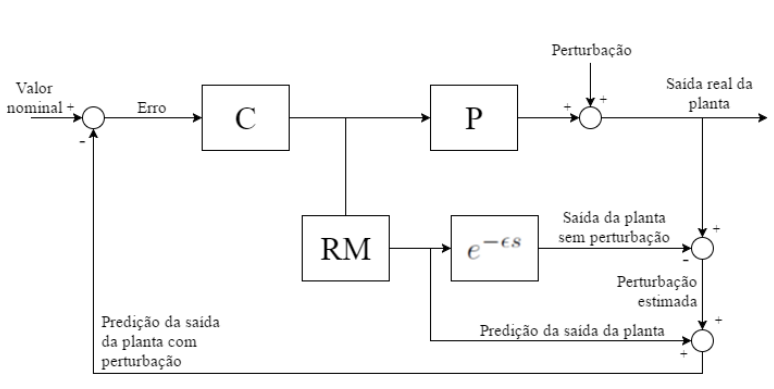
\includegraphics[width=.75\linewidth]{figures/smith/smith1}
\caption{Estrutura básica do preditor de Smith \cite{rafaelMestrado}}
\label{smithStruct1}
\end{figure}
\end{frame}

\begin{frame}[fragile]{Estrutura do Preditor de Smith com Filtro de Kalman}
Na Figura \ref{smithStruct2}, \textbf{P} é a planta, \textbf{C} é o controlador, \textbf{RM} é o modelo reduzido sem atraso, \textbf{KF} é o Filtro de Kalman e $e^{-\epsilon s}$ é o atraso puro. A nova estrutura considera referências das trajetórias de topo e de fundo.
\begin{figure}[!ht]
\centering
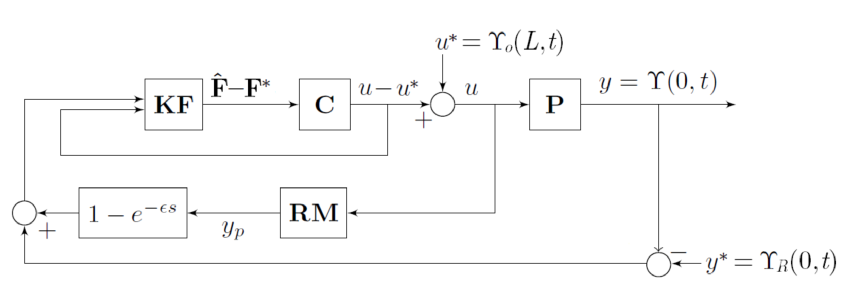
\includegraphics[width=.85\linewidth]{figures/smith/smith2}
\caption{Estrutura do preditor de Smith com Filtro de Kalman \cite{rafaelMestrado}}
\label{smithStruct2}
\end{figure}
\end{frame}

\begin{frame}[fragile]{Filtro de Kalman}
\begin{block}{Considerações sobre o Filtro de Kalman}
\begin{itemize}
\item Também conhecido como observador ótimo, é responsável por estimar variáveis de estado e a saída do sistema;
\item Utiliza uma estrutura de predição e correção para estimar as variáveis.
\end{itemize}
\end{block}
\end{frame}

\begin{frame}[fragile]{Filtro de Kalman - Modelagem}
O Filtro de Kalman pode ser aplicado em um sistema descrito por espaço de estados:
\begin{align}
\label{KalmanEq1}
	x_k &= \mathbf{A_k} x_{k-1} + \mathbf{B_k} u_k + w_{k-1}, \\
	\label{KalmanEq2}
	y_k &= \mathbf{C_k} x_k, \\
	\label{KalmanEq3}
	\tilde{y}_k &= y_k + v_k.
\end{align}
\begin{itemize}
\item $w_k$ e $v_k$ são ruídos relativos, respectivamente, ao processo e à medida;
\item $\tilde{y}_k$ é uma medida da saída do sistema.
\end{itemize}
\end{frame}

\begin{frame}[fragile]{Filtro de Kalman - Modelagem}
\begin{block}{Predição}
Nessa parte, é calculado o erro de covariância e o estado atual. Matematicamente:

\begin{align}
\label{KalmanEq4} {\hat{x}_{k}}^{-} &= \mathbf{A_k} \hat{x}_{k-1} + \mathbf{B_k} u_k\;\mathrm{e} \\
	\label{KalmanEq5} \mathbf{{\hat{P}_{k}}^{-}} &= \mathbf{A_k}\mathbf{P_{k-1}}\mathbf{{A_k}^T} + \mathbf{Q_k},
\end{align}

\begin{itemize}
\item $\hat{x}_{k}$ é a estimação das variáveis de estado;
\item $\mathbf{P_k}$ é a covariância do erro de medição, com estimação $\mathbf{{\hat{P}_{k}}}$;
\item $\mathbf{Q_k}$ é a covariância do ruído de processo.
\end{itemize}

\end{block}

\end{frame}

\begin{frame}[fragile]{Filtro de Kalman - Modelagem}
\begin{block}{Correção}
Nessa parte, o estado calculado na predição é corrigido incorporando-se uma medição mais recente do processo. Matematicamente:
\begin{align}
\label{KalmanEq6} \mathbf{K_k} &= \mathbf{{\hat{P}_{k}}^{-}}\mathbf{{C_k}^T} {\left( \mathbf{C_k}\mathbf{{\hat{P}_{k}}^{-}}\mathbf{{C_k}^T} + \mathbf{R_k} \right)}^{-1}, \\
	\label{KalmanEq7} \hat{x}_k &= {\hat{x}_{k}}^{-} + \mathbf{K_k} \left( \tilde{y}_k - \mathbf{C_k}{\hat{x}_{k}}^{-} \right)\;\mathrm{e} \\
	\label{KalmanEq8} \mathbf{P_k} &= \left( \mathbf{I} - \mathbf{K_k}\mathbf{C_k}\right)\mathbf{{\hat{P}_{k}}^{-}}.
\end{align}
\begin{itemize}
\item $\mathbf{K_k}$ é o ganho de Kalman;
\item $\mathbf{R_k}$ é a covariância do ruído de medida.
\end{itemize}
\end{block}
\end{frame}

\begin{frame}[fragile]{Bancada - Esquemático}
\begin{figure}[!ht]
	\centering
	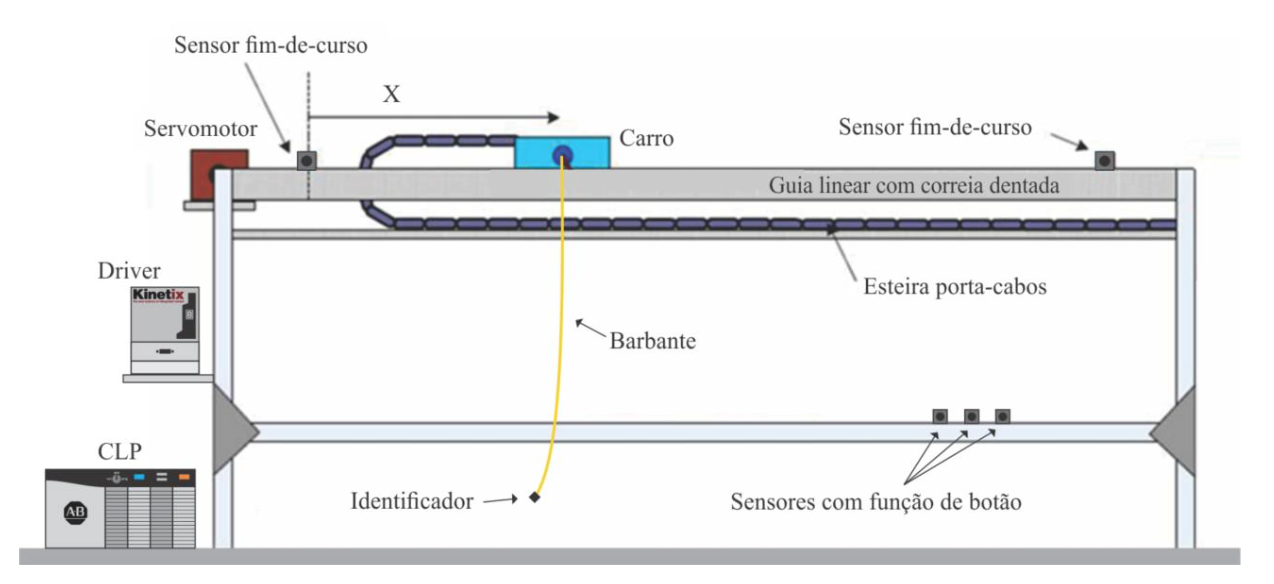
\includegraphics[width=.9\linewidth]{figures/fundamentos/bancadaEsquematico}
	\caption{Esquemático da ponte rolante \cite{redytton}}
	\label{bancadaesq}
\end{figure}
\end{frame}

\begin{frame}[fragile]{Bancada - Controlador}
\begin{block}{}
Responsável por receber dados da câmera e dos sensores, processá-los e enviar sinais de controle para o motor. Suporta várias linguagens de programação; para este projeto, foram utilizados \textit{ladder} e texto estruturado.
\end{block}
\begin{figure}[!ht]
	\centering
	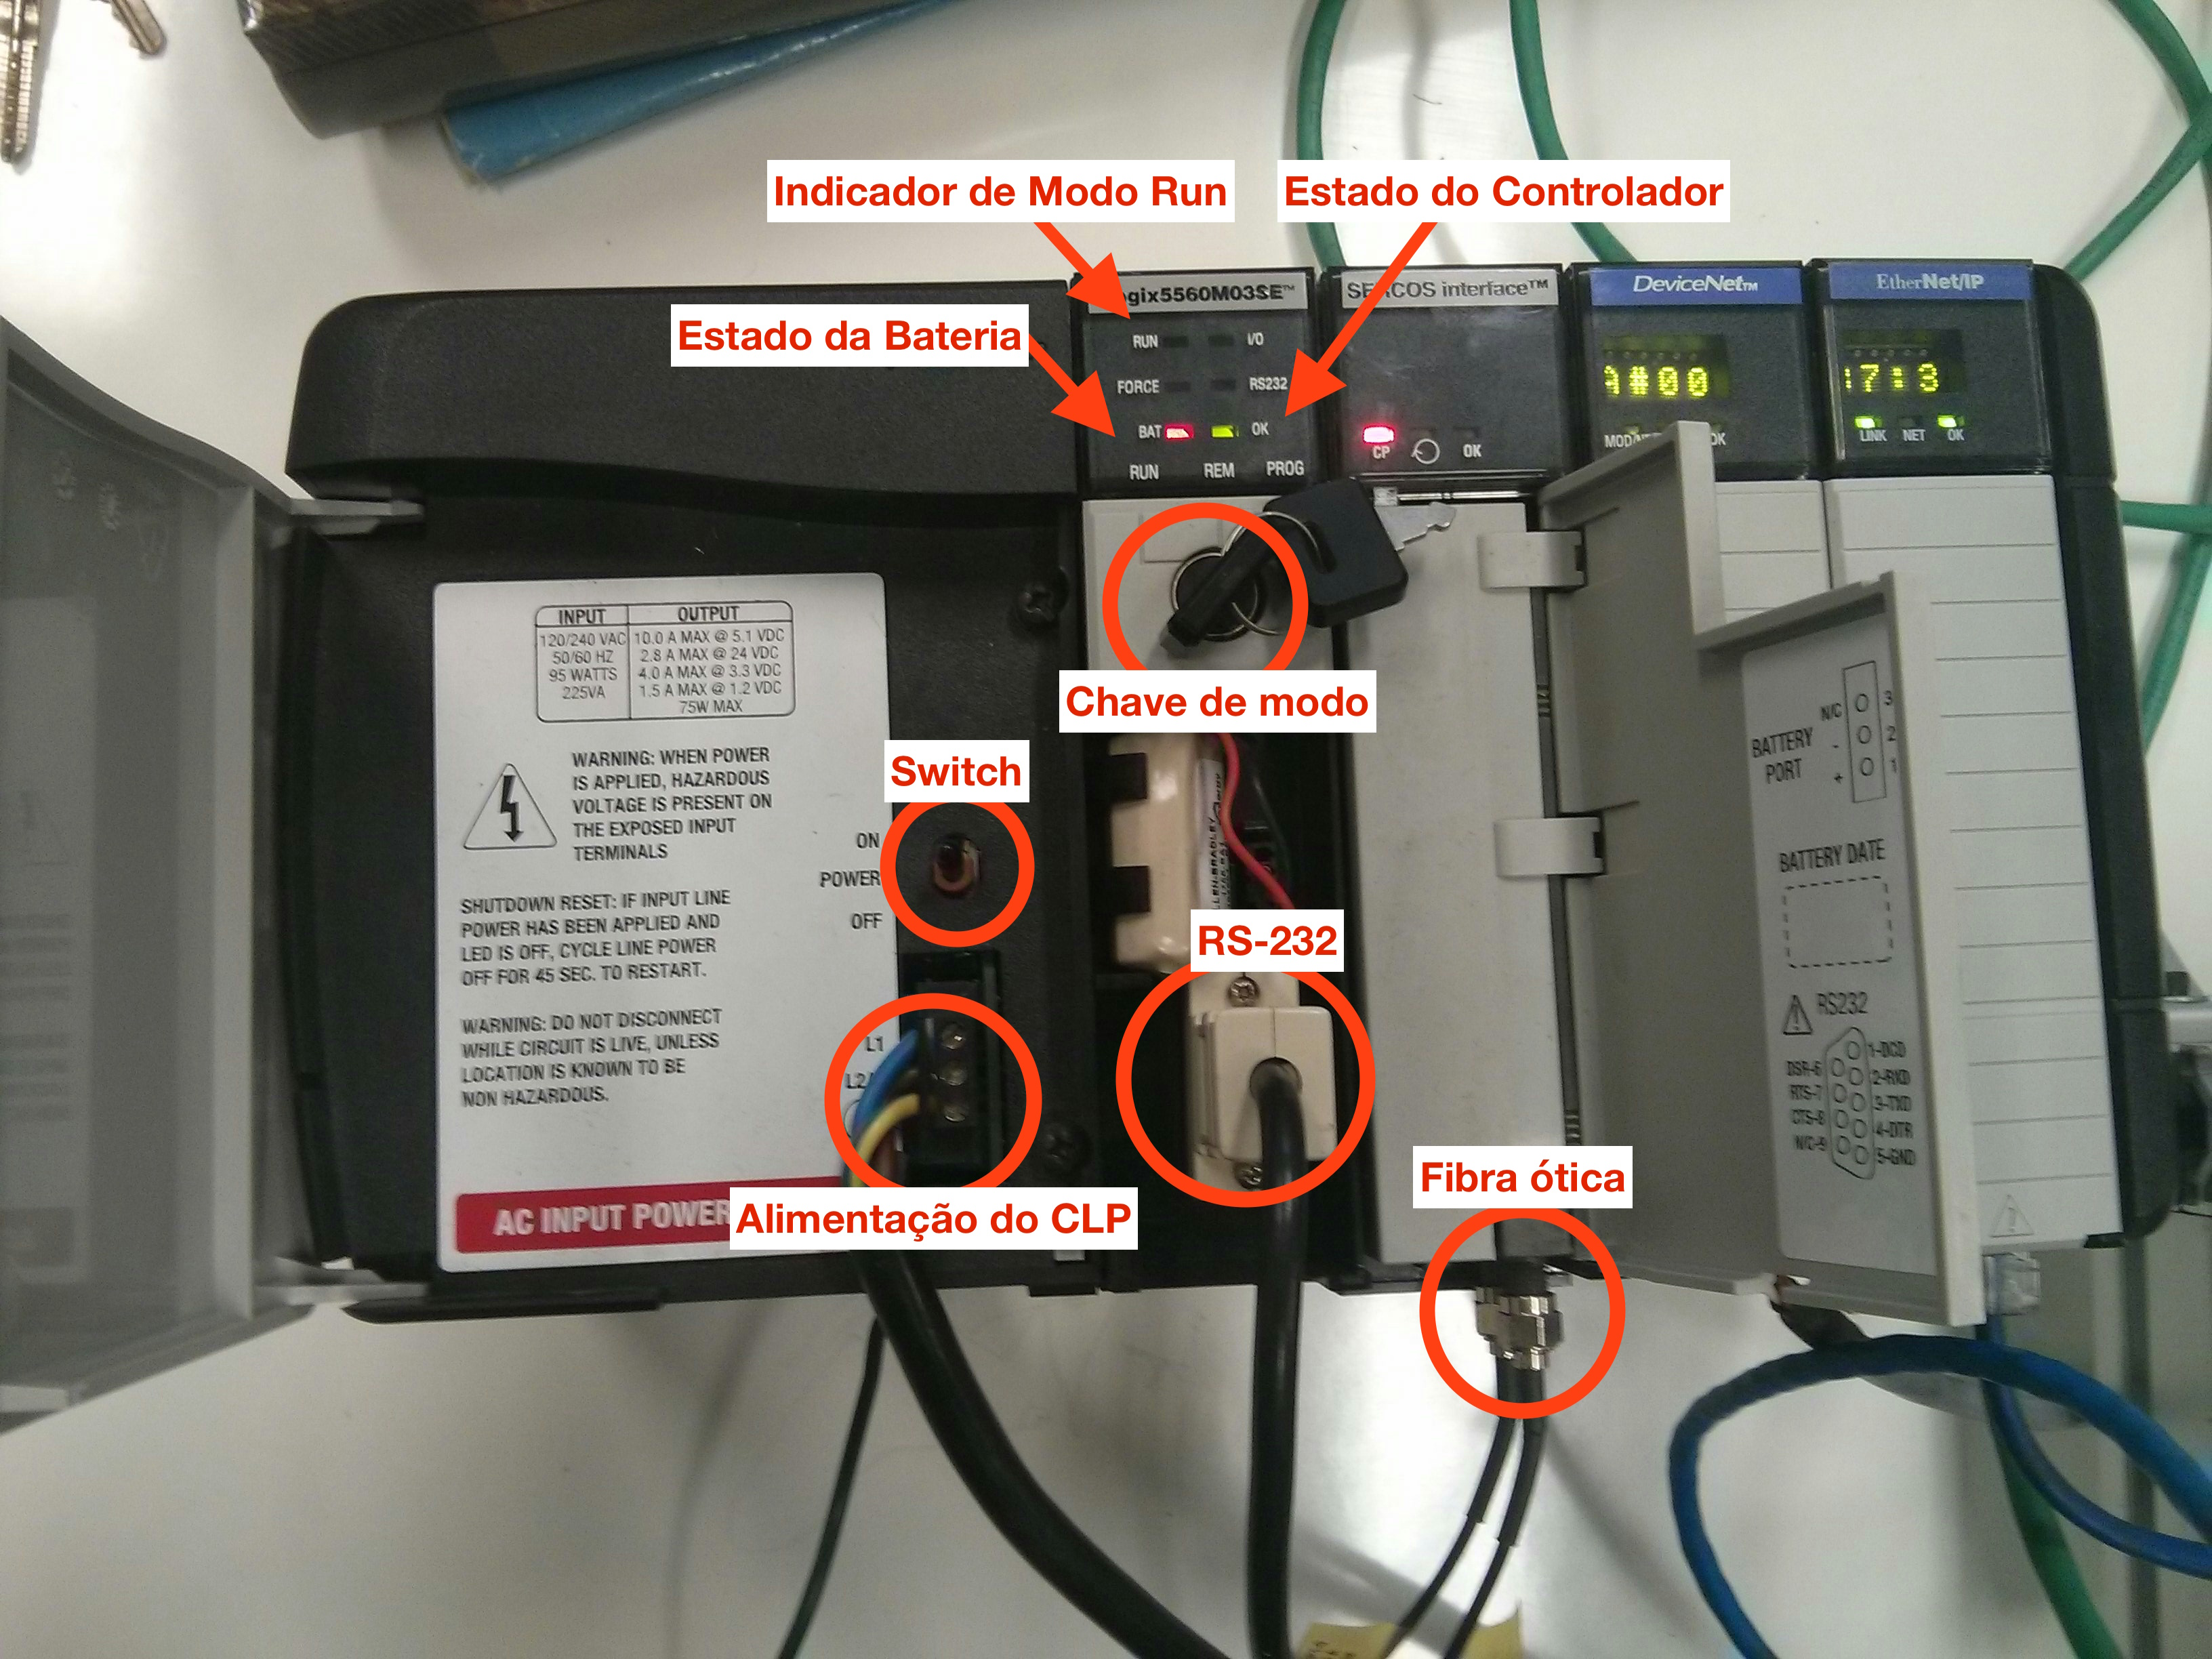
\includegraphics[width=.5\linewidth]{figures/fundamentos/CLP}
	\caption{Controlador Lógico Programável da \textit{Allen-Bradley}}
	\label{clpfig}
\end{figure}
\end{frame}

\begin{frame}[fragile]{Bancada - Câmera e Drive Kinetix}
\begin{columns}[T]

\begin{column}{.5\textwidth}
\begin{block}{Câmera}
Responsável por enviar a posição da bolinha para o CLP. Atua como sensor visual.
\end{block}

\begin{figure}[!ht]
	\centering
	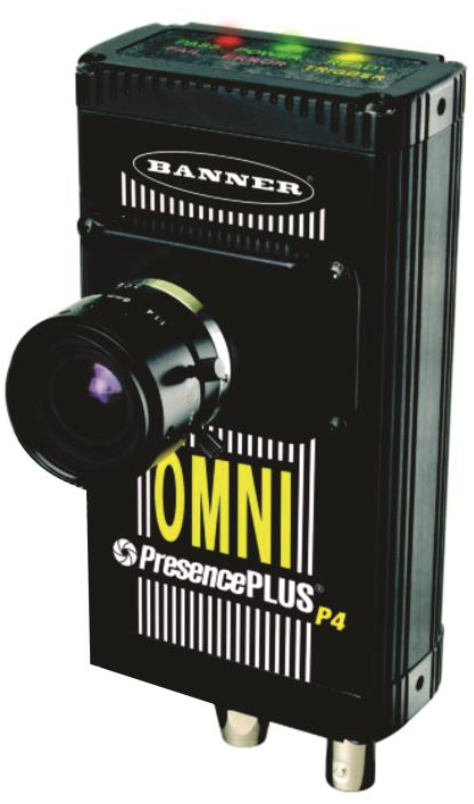
\includegraphics[width=.3\linewidth]{figures/fundamentos/camera}
	\caption{Câmera \textit{Presence Plus} \cite{redytton}}
	\label{bancadacamera}
\end{figure}

\end{column}

\begin{column}{.5\textwidth}

\begin{block}{Drive Kinetix}
Responsável por fornecer potência para o motor e controlá-lo por meio de pulsos PWM.
\end{block}

\begin{figure}[!ht]
	\centering
	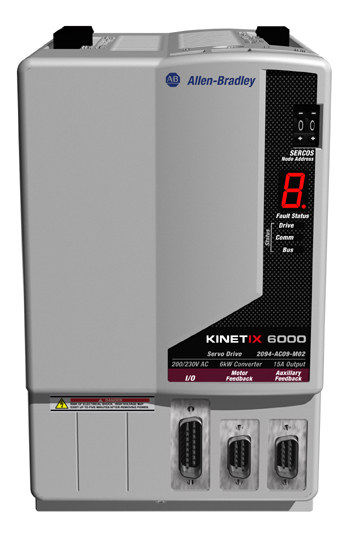
\includegraphics[width=.3\linewidth]{figures/fundamentos/kinetix6000}
	\caption{\textit{Drive Kinetix 6000} \cite{redytton}}
	\label{bancadadrive}
\end{figure}

\end{column}

\end{columns}
\end{frame}

\begin{frame}[fragile]{Bancada - \textit{Line Interface Module}}
\begin{block}{}
Responsável pela interface elétrica entre o \textit{Drive Kinetix} e a rede de alimentação trifásica.
\end{block}

\begin{figure}[!ht]
	\centering
	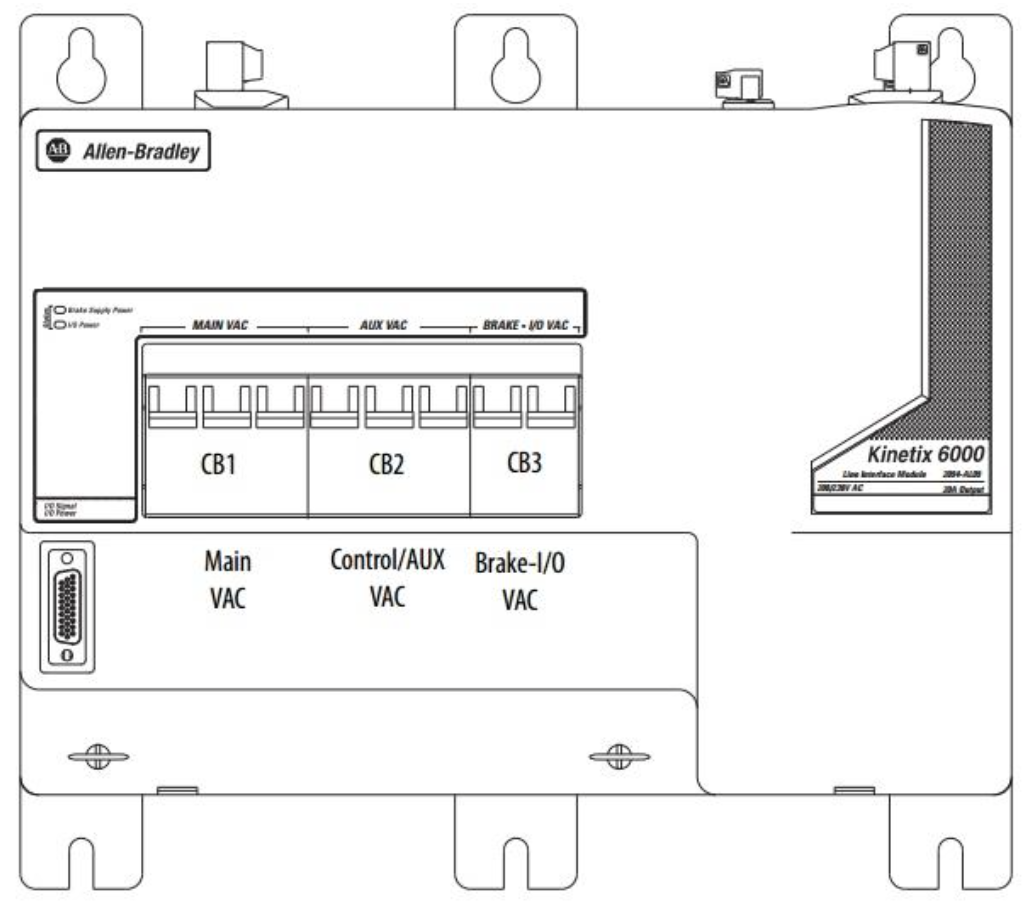
\includegraphics[width=.5\linewidth]{figures/fundamentos/LineInterfaceModule}
	\caption{\textit{Line Interface Module} \cite{redytton}}
	\label{bancadalim}
\end{figure}

\end{frame}

\begin{frame}[fragile]{Bancada - Sensores Indutivos e Servomotor}

\begin{columns}[T]

\begin{column}{.5\textwidth}

\begin{block}{Sensores Indutivos}
Detectam objetos metálicos; podem operar em modo analógico ou digital. Utilizados como chaves de fim de curso para a rotina de emergência.
\end{block}

\begin{figure}[!ht]
	\centering
	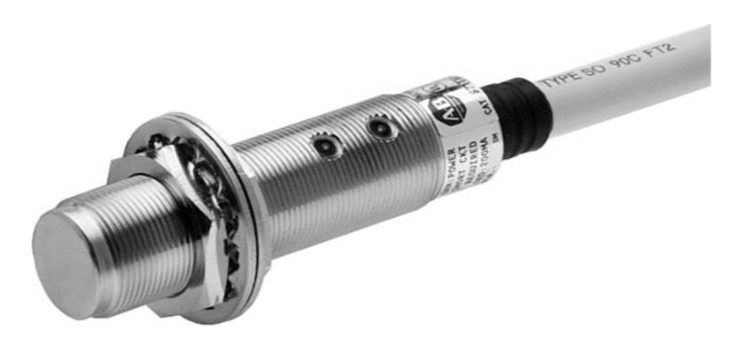
\includegraphics[width=.6\linewidth]{figures/fundamentos/sensorIndutivo}
	\caption{Sensor Indutivo \cite{redytton}}
	\label{bancadaindut}
\end{figure}

\end{column}

\begin{column}{.5\textwidth}

\begin{block}{Servomotor}
Atuador rotatório composto de motor elétrico com sensor acoplado; permite controle preciso da posição angular.
\end{block}

\begin{figure}[!ht]
	\centering
	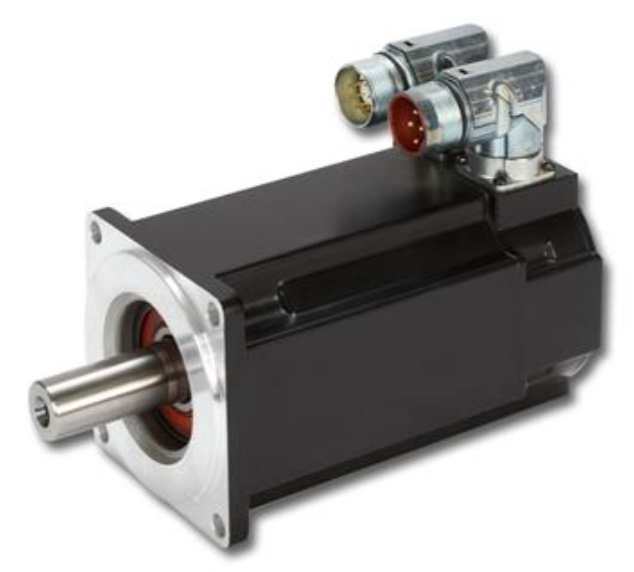
\includegraphics[width=.5\linewidth]{figures/fundamentos/servomotor}
	\caption{Servomotor \cite{redytton}}
	\label{bancadaservo}
\end{figure}

\end{column}

\end{columns}

\end{frame}

\begin{frame}[fragile]{Redes Industriais}
\begin{columns}[T]
\begin{column}{.5\textwidth}
\begin{block}{DeviceNet}
Rede responsável por conectar os sensores indutivos ao CLP por meio do módulo 1756-DNB. Suporta conexões de dispositivos de baixo nível com CLPs e outros dispositivos de alto nível, como o computador \cite{devicenetrockwell}. O módulo responsável pelo \textit{scan} desta rede é o \textit{1756-DNB}.
\end{block}
\end{column}

\begin{column}{.5\textwidth}
\begin{block}{Ethernet/IP}
Transmite dados da câmera para o CLP, e também transfere os programas em \textit{ladder} ou texto estruturado do computador para o controlador. É uma rede indicada para aplicações em que o tempo é crítico \cite{eiprockwell}. O módulo responsável pelo \textit{scan} desta rede é o \textit{1756-ENBT/A}.
\end{block}
\end{column}

\end{columns}
\end{frame}

\begin{frame}[fragile]{Redes Industriais}
\begin{block}{OPC - \textit{OLE for Process Control}}
Responsável pelo compartilhamento de dados entre o CLP e outros \textit{softwares} no computador. Utilizado para se efetuar atualização de dados dentro do CLP, mas fora do \textit{software} RSLogix5000. Desta forma, partes do controle da bancada podem ser escritos, por exemplo, em Python.
\end{block}
\end{frame}


\begin{frame}[fragile]{Parâmetros Para Geração de Trajetórias}
\begin{table}[!ht]
\centering
\caption{Dados para simulação em escala real\label{escalaReal} \cite{redytton}}
	\begin{tabular}{|c|c|}
	\hline
		\multicolumn{2}{|c|}{\textbf{Dados do Riser}}\\ \hline
		Diâmetro externo & $0.55\mathrm{m}$\\ \hline
		Diâmetro interno & $0.5\mathrm{m}$ \\ \hline
		Comprimento & $2000\mathrm{m}$ \\ \hline
		Módulo de Elasticidade & $200 \mathrm{GPa}$\\ \hline
		Densidade &  $7860\mathrm{kg}/\mathrm{m}^3$\\ \hline
		\multicolumn{2}{|c|}{\textbf{Dados do fluido (Água)}}\\ \hline
		Densidade do fluido &  $1000\mathrm{kg}/\mathrm{m}^3$\\ \hline
		Viscosidade dinâmica & $10^3 \mathrm{Pa}\cdot \mathrm{s}$ \\ \hline
	\end{tabular}



\end{table}

\end{frame}

\begin{frame}[fragile]{Parâmetros Para Geração de Trajetórias}

\begin{table}[!ht]
	\caption{Dados para simulação em escala laboratorial\label{escalaLaboratorial}}
	\centering
	\begin{tabular}{|c|c|}
		\hline
			\multicolumn{2}{|c|}{\textbf{Dados da Massa na Ponta - Isopor}} \\ \hline
			Diâmetro Externo & $30.6\mathrm{mm}$\\ \hline
			Densidade & $10\mathrm{kg}/\mathrm{m}^3$ \\ \hline
			\multicolumn{2}{|c|}{\textbf{Dados do Riser (Barbante)}}\\ \hline
			Diâmetro externo & $2\mathrm{mm}$\\ \hline
			Diâmetro interno & $0\mathrm{mm}$ \\ \hline
			Comprimento & $82\mathrm{cm}$ \\ \hline
			Módulo de Elasticidade & $2.1 \mathrm{MPa}$\\ \hline
			Densidade &  $191\mathrm{kg}/\mathrm{m}^3$\\ \hline
			\multicolumn{2}{|c|}{\textbf{Dados do fluido (Ar)}}\\ \hline
			Densidade do fluido &  $1.2754\mathrm{kg}/\mathrm{m}^3$\\ \hline
			Viscosidade dinâmica & $17.2\cdot 10^6 \mathrm{Pa}\cdot \mathrm{s}$ \\ \hline
		\end{tabular}
\end{table}

\end{frame}


\section{Resultados}

\begin{frame}[fragile]{Calibração da Câmera}
\begin{block}{Passos para a calibração da câmera}
\begin{enumerate}
	\item Atualização do \textit{firmware};
	\item Reconhecimento da câmera pelo \textit{software RsLinx};
	\item Estabelecimento de um endereço IP para a câmera no \textit{software PresencePlus};
	\item Uso das ferramentas de tomada de dados da câmera no \textit{software PresencePlus};
	\item Obtenção da relação entre \textit{pixels} da câmera e milímetros.
\end{enumerate}
\end{block}
\end{frame}

\begin{frame}[fragile]{Calibração da Câmera}
\begin{block}{Ferramentas utilizadas}
\begin{itemize}
	\item \texttt{Locate}: Localiza o corpo desejado pelas bordas;
	\item \texttt{Geometric}: Localiza o ``centro geométrico'' do corpo a ser detectado;
	\item \texttt{Measure}: Responsável por efetuar medições em \textit{pixels} entre pontos de referência desejados;
	\item \texttt{Math}: Executa cálculos matemáticos;
	\item \texttt{Communication}: Transfere os dados de interesse da câmera para o CLP por meio da rede Ethernet/IP.
\end{itemize}
\end{block}
\end{frame}

\begin{frame}[fragile]{Calibração da Câmera - Reconhecimento do \textit{Software RSLinx}}
\begin{figure}[!ht]
\centering
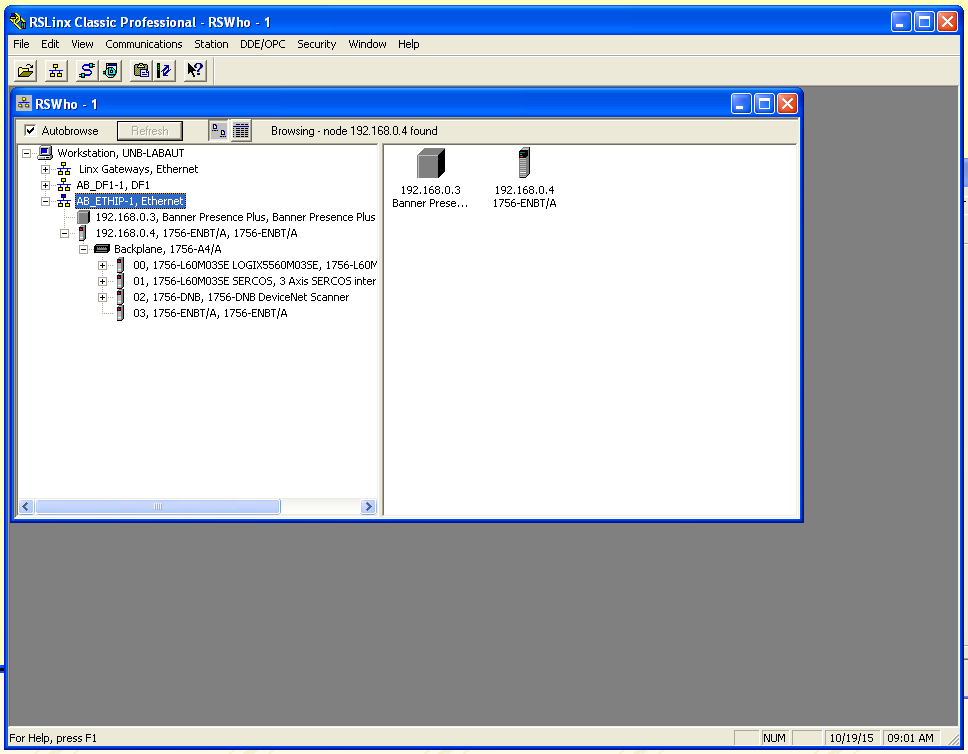
\includegraphics[width=.7\linewidth]{figures/resultados/camera/cameralinx}
\caption{\textit{RSLinx} com câmera reconhecida \label{linxcamera}}
\end{figure}
\end{frame}

\begin{frame}[fragile]{Calibração da Câmera - Configuração do Módulo Ethernet/IP}
\begin{figure}[!ht]
\centering
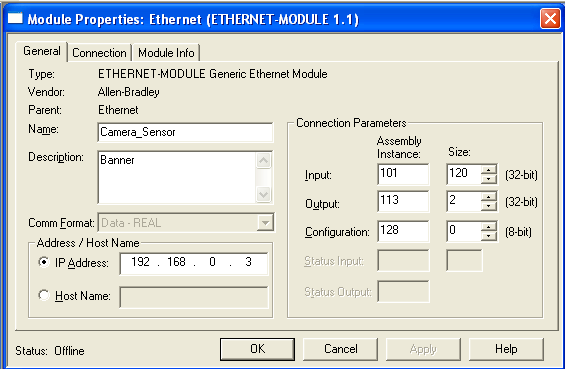
\includegraphics[width=.8\linewidth]{figures/resultados/camera/cameraSetup}
\caption{Configuração do módulo 1756-ENBT para uso dos dados da câmera\label{setupcamera}}
\end{figure}
\end{frame}

\begin{frame}[fragile]{Calibração da Câmera - \textit{Software PresencePlus}}
\begin{figure}[!ht]
\centering
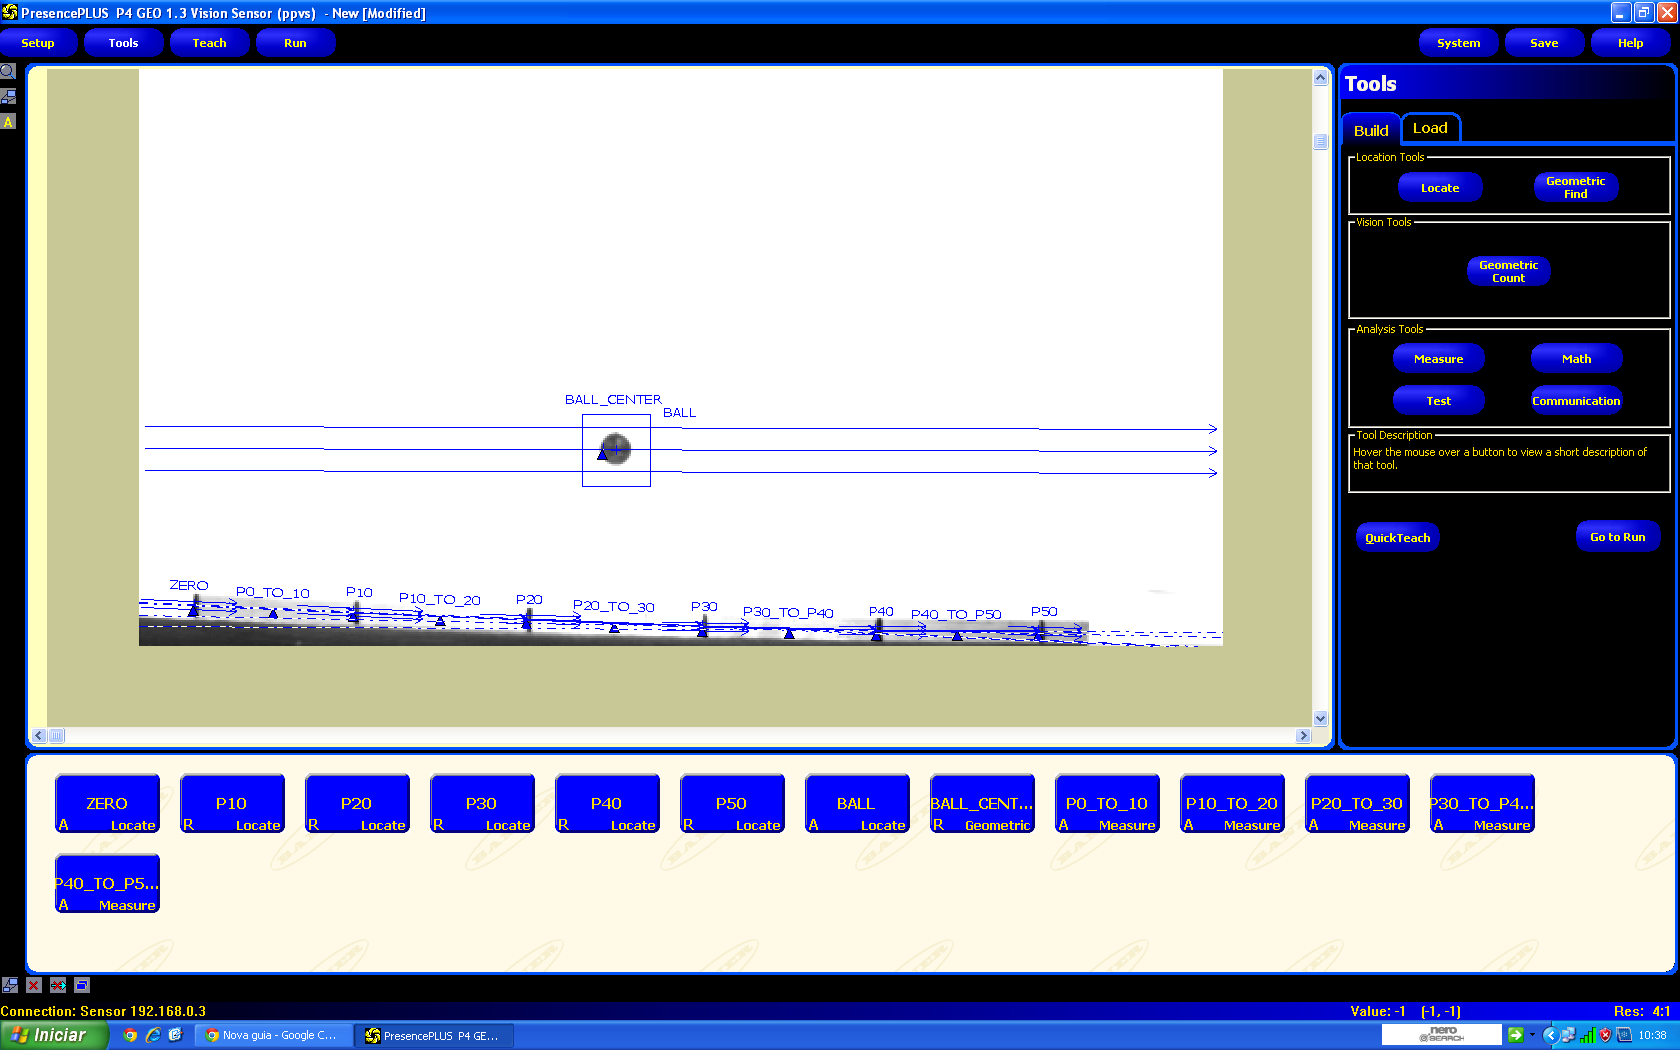
\includegraphics[width=.9\linewidth]{figures/resultados/camera/programa}
\caption{Calibração da câmera pelo \textit{software PresencePlus} \label{calibcamera}}
\end{figure}
\end{frame}

\begin{frame}[fragile]{Calibração da Câmera - Resultados}
\begin{table}[!ht]
\centering
\caption{Relações mm/px para diferentes seções da barra de alumínio \label{relacoesmmpx}}
	\begin{tabular}{|c|c|c|c|}
	\hline
		Seção 1 & Seção 2 & Distância (px) & mm/px\\ \hline
		P0 & P10 & 160 & 0.625\\ \hline
		P10 & P20 & 173 & 0.578\\ \hline
		P20 & P30 & 176 & 0.568\\ \hline
		P30 & P40 & 173 & 0.578\\ \hline
		P40 & P50 & 163 & 0.613\\ \hline
		P0 & PEND & 893 & 0.596\\ \hline
	\end{tabular}
\end{table}
Erro aproximado: 4.93 \%
\end{frame}

\begin{frame}[fragile]{Calibração do Servomotor}
\begin{block}{Passos para a calibração}
\begin{enumerate}
	\item Obtenção da posição inicial $x_0$ e posição final $x_f$, em milímetros;
	\item Definição de um intervalo de tempo $\Delta t$ e uma velocidade de movimentação do carrinho $v$ em $[\mathrm{u}/\mathrm{s}]$;
	\item Cálculo da velocidade em $[\mathrm{mm}/\mathrm{s}]$ a partir dos dados obtidos.
\end{enumerate}
\end{block}
\end{frame}

\begin{frame}[fragile]{Calibração do Servomotor - Resultados}

\begin{table}[!ht]
\centering
\caption{Dados de calibração do servomotor, média obtida é de 71.32 mm/unidade\label{calibracaoServomotor}}
\resizebox{\textwidth}{!}{
\begin{tabular}{|c|c|c|c|c|c|}
\hline
	$x_0$ - [mm] & $x_f$ - [mm] & $\Delta t$ - [s] & Velocidade - [u/s] & Velocidade - [mm/s] & mm/u\\ \hline
2 &	71.8  &	2   &	0.5 &	34.9   & 	69.8\\ \hline
6 & 76.1  &	2   &	0.5 &	35.05  &	70.1\\ \hline
6 &	188	  &  5   &	0.5	&   36.4   &	72.8\\ \hline
6 &	185   &	2.5 &	1	& 	71.6   &	71.6\\ \hline
6 &	77    &	10  &	0.1	&   7.1    &	71\\ \hline
6 &	296.5 &	20	&   0.2 & 	14.525 &	72.625\\ \hline\end{tabular}
}
\end{table}

\end{frame}

\begin{frame}[fragile]{Testes utilizando trajetória Rampa}
\begin{columns}[T]
\begin{column}{.5\textwidth}
\begin{figure}[!ht]
\centering
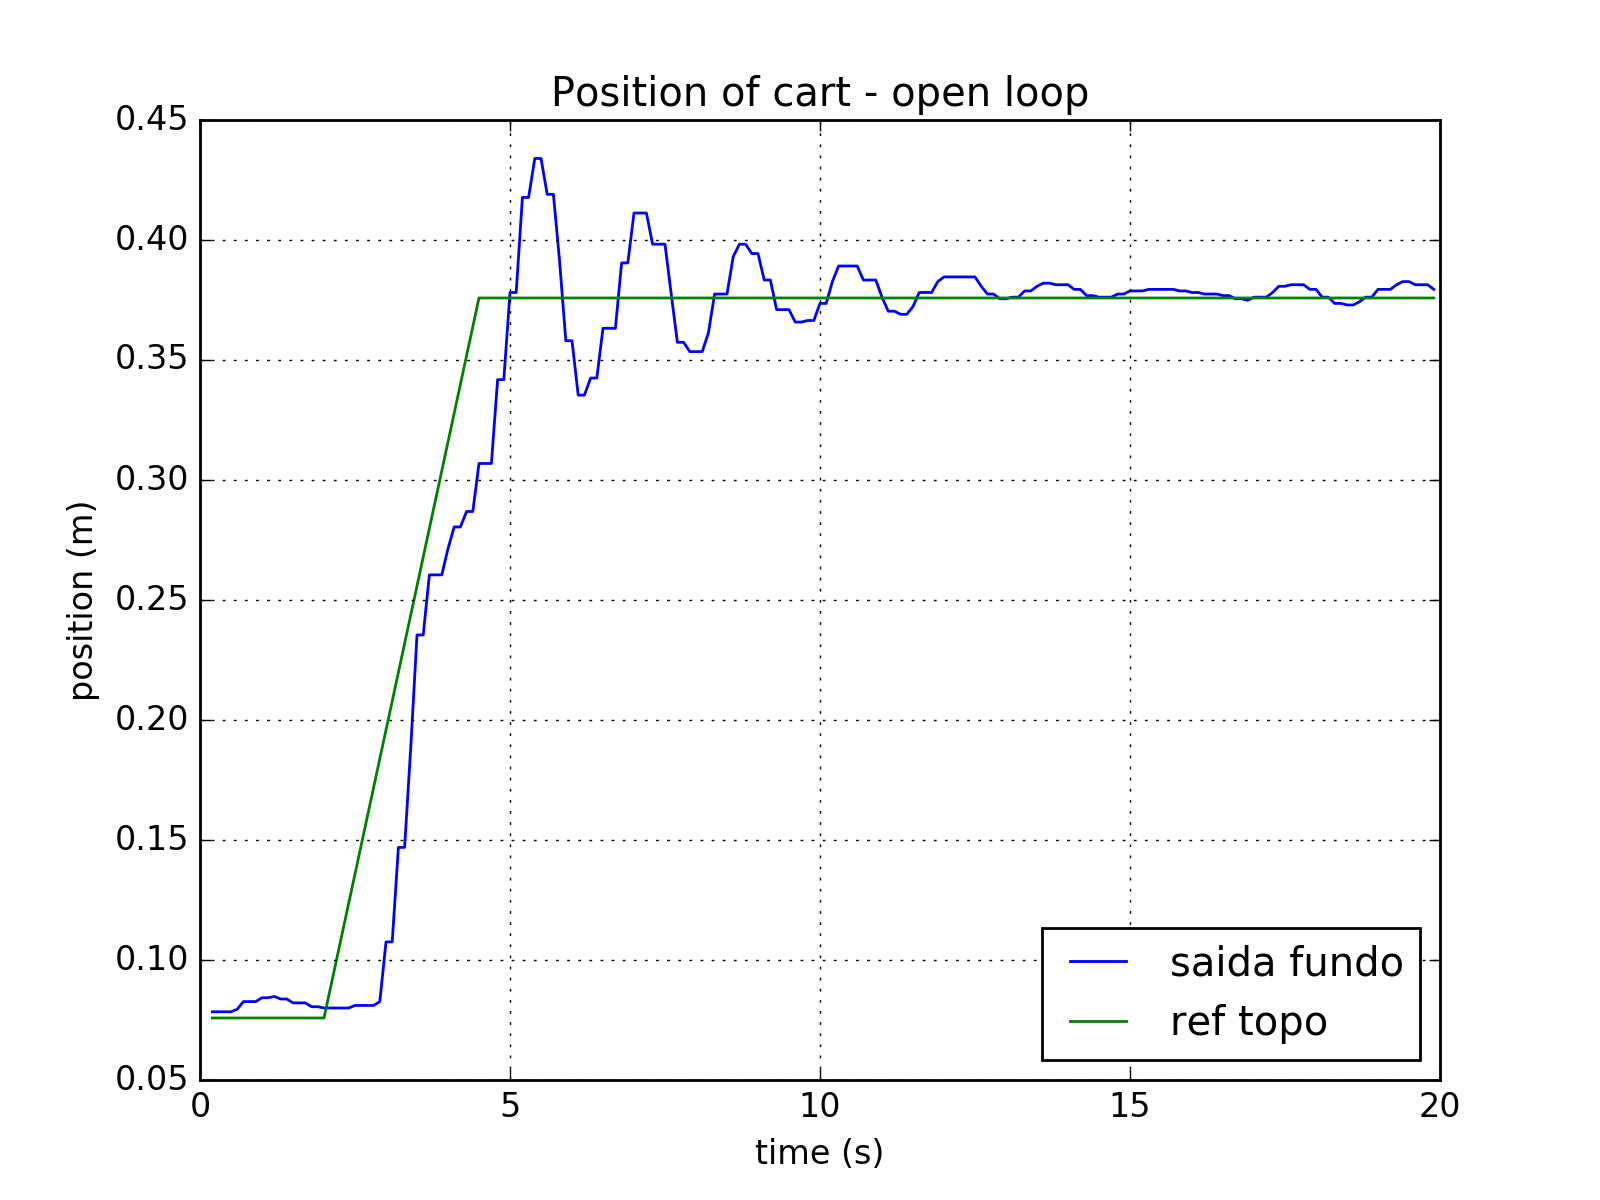
\includegraphics[width=1\textwidth]{figures/resultados/experimento/open_loop_ramp}
\caption{Teste com rampa em malha aberta}
\label{openLoopRamp}
\end{figure}
\end{column}

\begin{column}{.5\textwidth}
\begin{figure}[!ht]
\centering
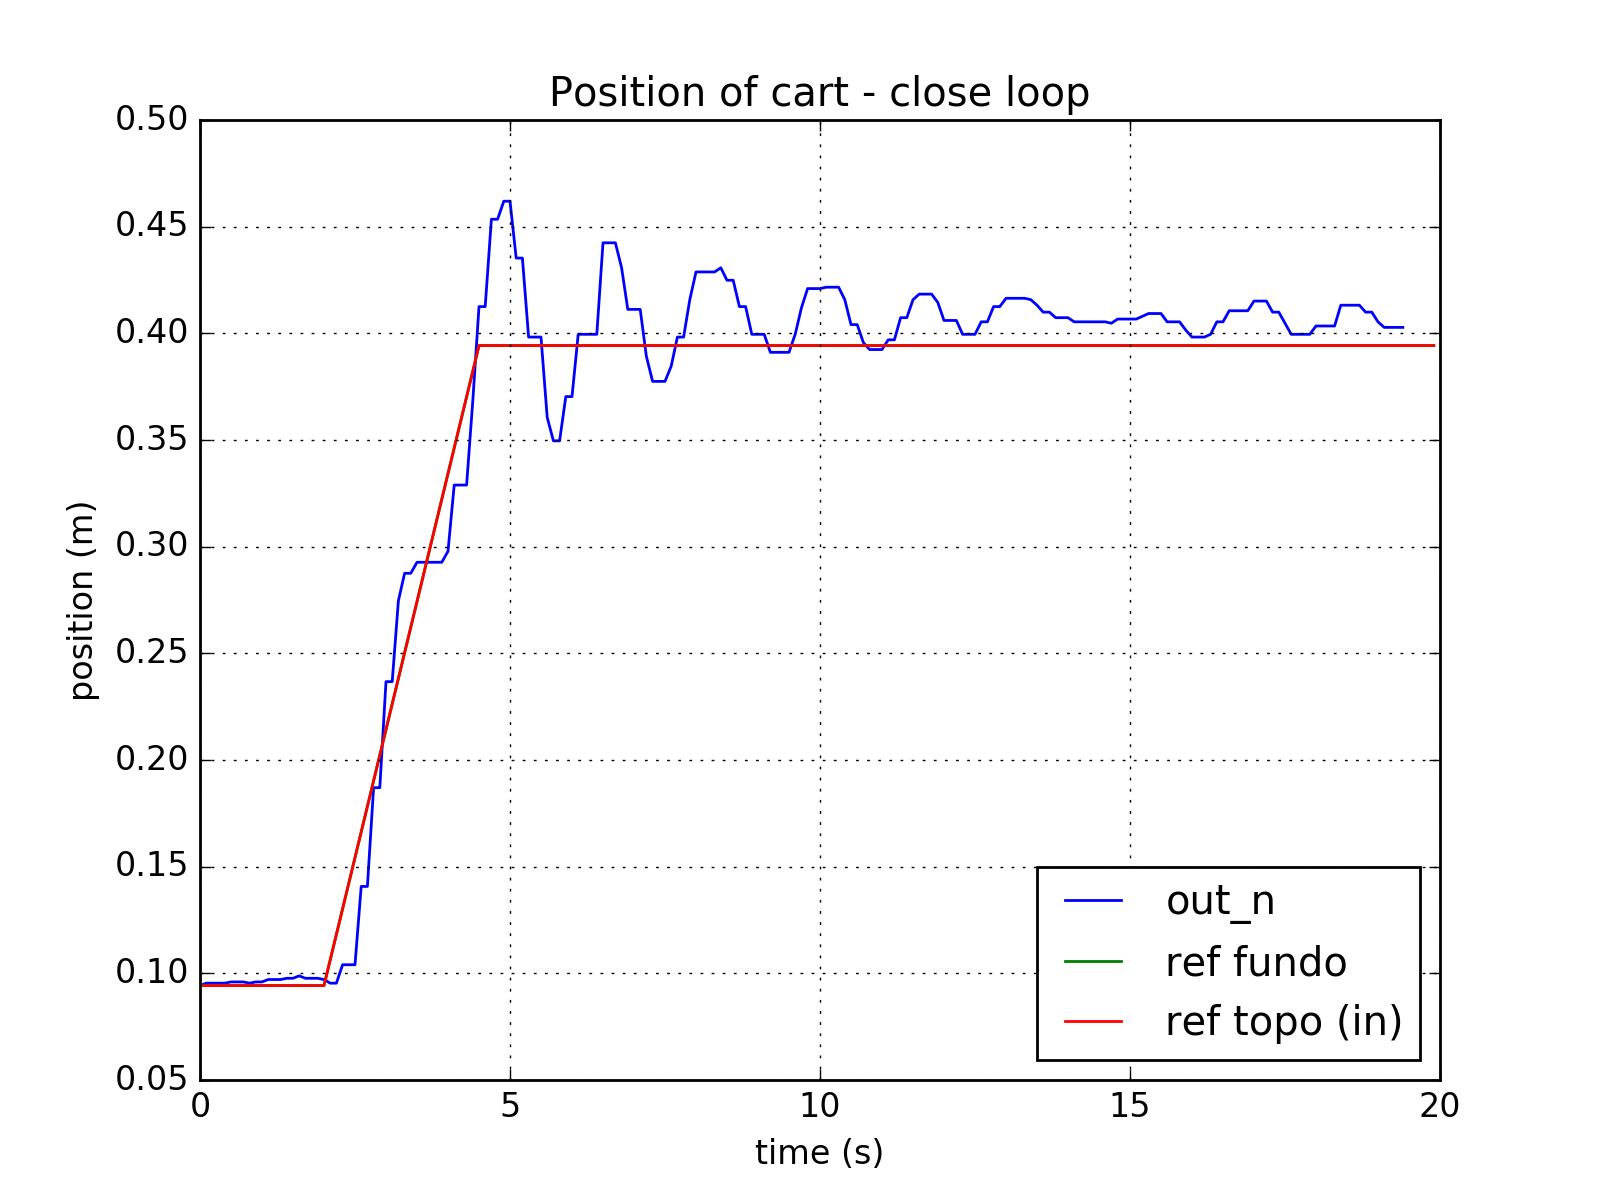
\includegraphics[width=1\textwidth]{figures/resultados/experimento/closed_loop_trajetoria_rampa}
\caption{Teste com rampa usando Preditor de Smith}
\label{closedLoopRamp}
\end{figure}
\end{column}
\end{columns}
\end{frame}

\begin{frame}[fragile]{Testes utilizando trajetória Rampa}
\begin{figure}[!ht]
\centering
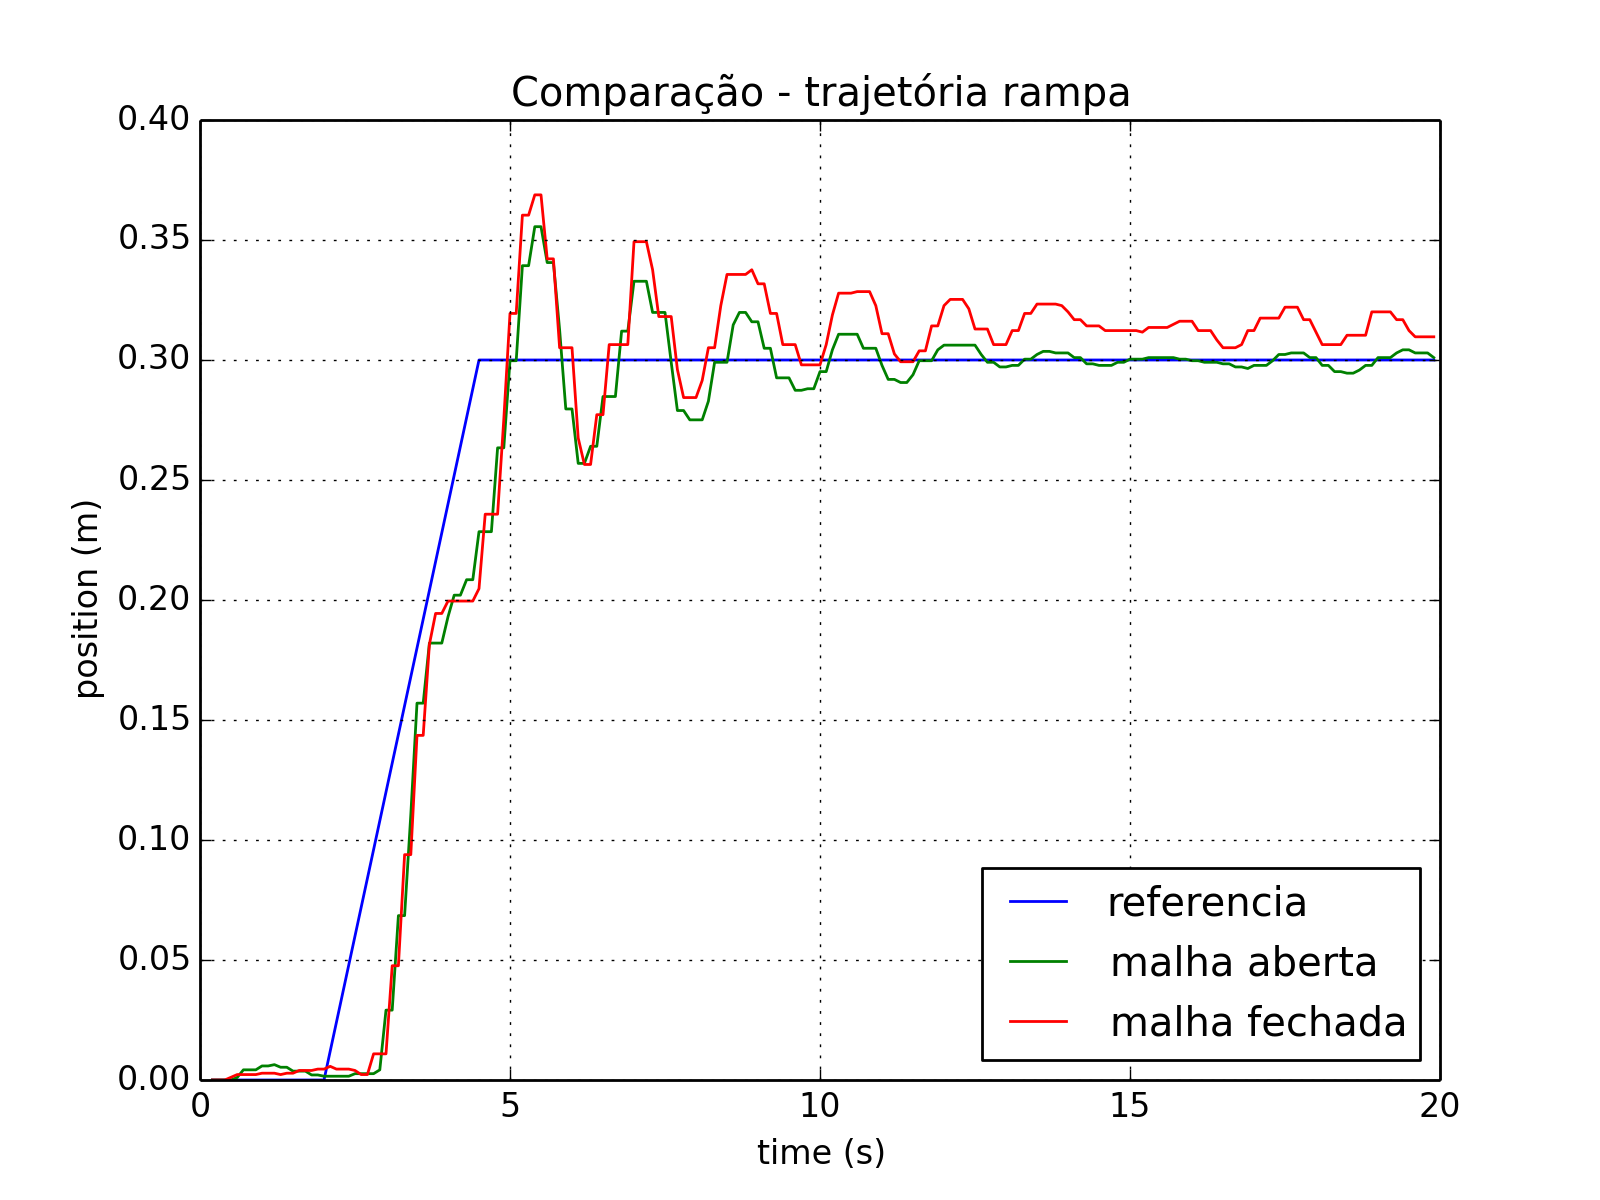
\includegraphics[width=.8\linewidth]{figures/resultados/experimento/rampa_comp}
\caption{Gráfico comparativo dos testes com rampa}
\label{rampaComp}
\end{figure}
\end{frame}

\begin{frame}[fragile]{Teste com Trajetória Suave de 30 cm}
\begin{figure}[!ht]
\centering
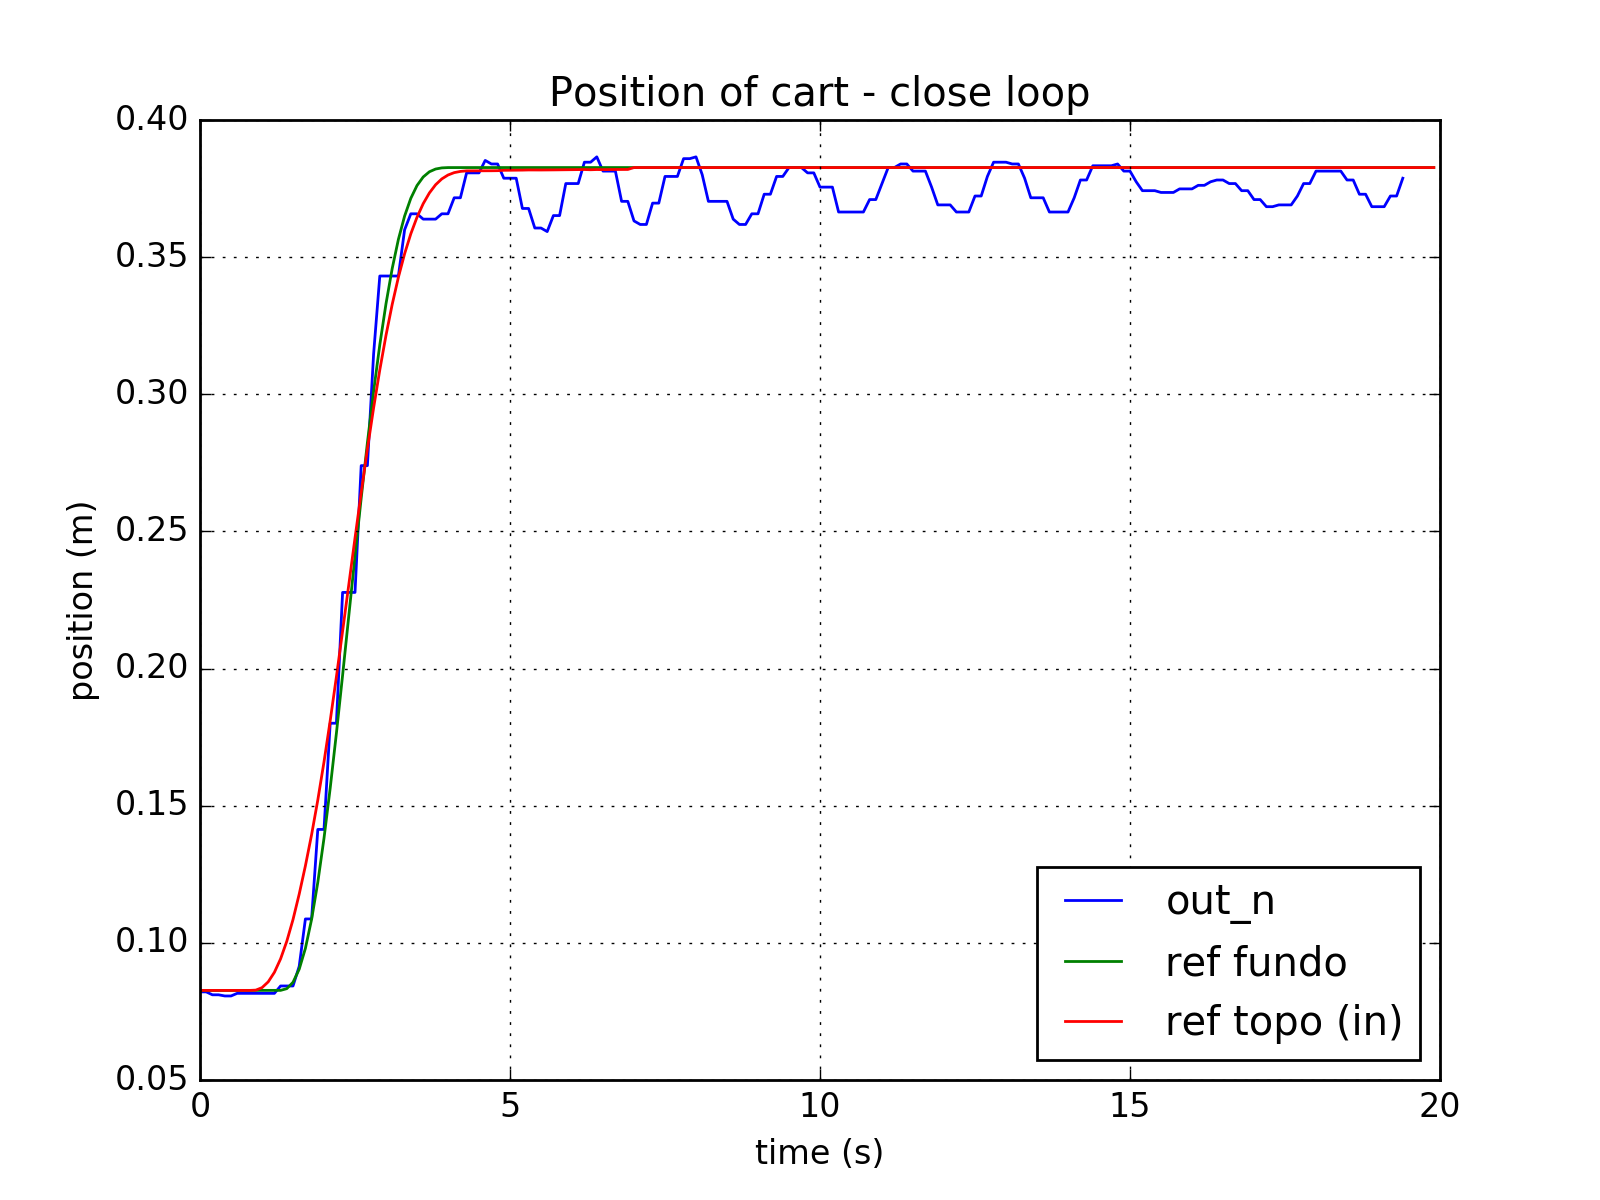
\includegraphics[width=.8\linewidth]{figures/resultados/experimento/closed_loop_trajetoria_rafael}
\caption{Teste com trajetória suave - 20 segundos}
\label{trajSuave20}
\end{figure}
\end{frame}

\begin{frame}[fragile]{Teste com Trajetória Suave de 30 cm - Detalhe}
\begin{figure}[!ht]
\centering
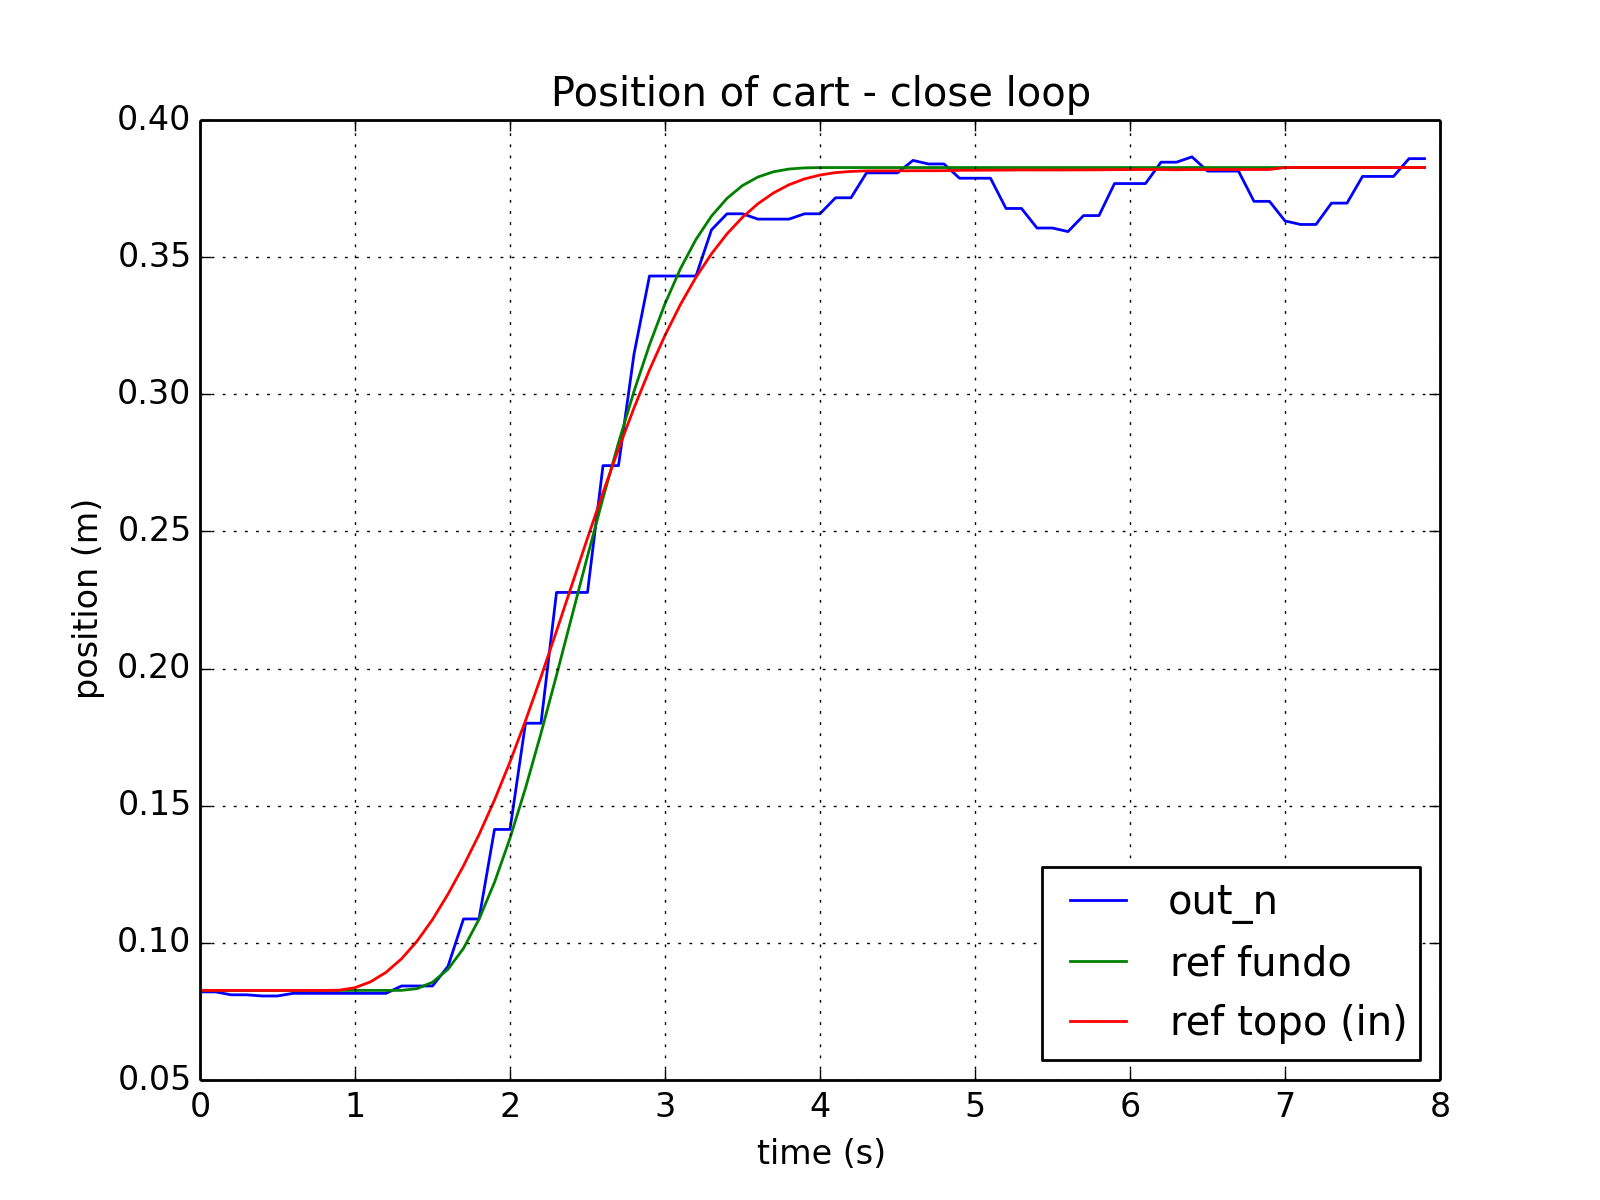
\includegraphics[width=.8\linewidth]{figures/resultados/experimento/closed_loop_trajetoria_rafael_detalhe}
\caption{Teste com trajetória suave - 8 segundos}
\label{trajSuave8}
\end{figure}
\end{frame}

\begin{frame}[fragile]{\textit{Links} Interessantes}
\begin{block}{\textit{Links} para vídeos com resultados}
\begin{enumerate}
	\item Teste com Rampa em Malha Aberta - \url{https://youtu.be/chrez0QEucU}
	\item Teste com Rampa usando Preditor - \url{https://youtu.be/QOuxlsT3gBA}
	\item Excursão 30 cm usando Preditor - \url{https://youtu.be/lpPZ7HOG7hM}
\end{enumerate}
\end{block}
\end{frame}

\section{Conclusão}

\begin{frame}[fragile]{Conclusão}
\begin{block}{Conclusões}
\begin{itemize}
	\item Foi possível desenvolver uma estrutura baseada no Preditor de Smith de forma a se controlar a trajetória do barbante de forma razoável; o sistema da ponte rolante foi reduzido para um sistema de ordem baixa, e foi utilizado o preditor em conjunção com Filtro de Kalman e controlador por realimentação de estados com canal integral para se efetuar o controle de trajetória;
	\item Pelos resultados experimentais, nota-se que é possível adaptar o preditor construído para a situação de um \textit{riser} real, efetuando-se as correções necessárias.
\end{itemize}
\end{block}
\end{frame}

\begin{frame}[fragile]{Conclusão}
\begin{block}{Perspectivas Futuras}
\begin{itemize}
	\item Aprimorar a calibração da câmera para permitir excursões maiores;
	\item Procurar métodos diferentes de controle e testar sua eficiência em relação ao Preditor de Smith;
	\item Melhorar a programação utilizada, tornando-a mais eficiente;
	\item Corrigir o Filtro de Kalman, e utilizar outros formatos do mesmo.
\end{itemize}
\end{block}
\end{frame}


\plain{Dúvidas?}

\begin{frame}[allowframebreaks]{Referências}

  \bibliography{apresentacaoTG2}
  \bibliographystyle{abbrv}

\end{frame}

\plain{Obrigado!}

\end{document}
